\documentclass{article}
\usepackage{nips12submit_e,times}
%\documentclass[10pt,twocolumn,fleqn]{article}
%\setlength{\columnsep}{0.25in}
%\usepackage{fullpage}
%\usepackage[margin=0.70in]{geometry}

\usepackage[square,numbers]{natbib}
\usepackage{amsmath, epsfig}
\usepackage{amsfonts}
\usepackage{graphicx}
\usepackage{amsfonts}
\usepackage{algorithm}
\usepackage{algorithmic}
\usepackage{easybmat}
\usepackage{footmisc}
\usepackage[usenames,dvipsnames]{color}
\usepackage{subfig}
\usepackage{hyperref}
\renewcommand\algorithmiccomment[1]{// \textit{#1}}
\newcommand{\ignore}[1]{}
\newcommand{\comment}[1]{}
\newcommand{\willie}[1]{\textcolor{red}{\textsf{\emph{\textbf{\textcolor{red}{#1}}}}}}
\DeclareMathOperator*{\argmax}{arg\,max}
\newcommand{\norm}[1]{\left|\left|#1\right|\right|}

\title{Embedding Nodes via their Local Network Topology for Role Descriptors in Social Networks}
%\title{Embedding Graph Vertices via Local Network Topology for Identifying Role-Types in Social Networks}

\author{
Willie Neiswanger\thanks{Anything here?} \\
School of Computer Science\\
Carnegie Mellon University\\
Pittsburgh, PA 15213 \\
\texttt{willie@cs.cmu.edu} \\
}

\newcommand{\fix}{\marginpar{FIX}}
\newcommand{\new}{\marginpar{NEW}}

%\nipsfinalcopy % Uncomment for camera-ready version

\begin{document}

\maketitle

\begin{abstract}
This paper proposes a method for characterizing the local network topology in the vicinity of each vertex in a graph. The method provides a Euclidean embedding of each node based on its local network structure. We show how descriptors of the local topologies of vertices can be used to quantify the types of local structure found in a network and identify groups of nodes with similar roles relative to nearby vertices. Our method for embedding makes use of the Fixed Node Edit Distance (FNED), a distance metric between the local topologies around nodes, which we define. We give multiple algorithms for computing the FNED given different graph structures, show how it can be used for embedding the local topologies of nodes in Euclidean space, and demonstrate the embedding on multiple publicly available network datasets. Results show the ability of this method to characterize diverse regions of network structure and identify groups of entities with similar roles in social networks.
\end{abstract}


\section{Introduction}
\label{sec:intro}

\section{Definitions}
\label{sec:defs}


\subsection{$k$-Step Local Topology of a Node}
Let $G = \{V,E\}$ be a graph with a set of vertices $V$ and edges $E$. We would like to capture the network topology around a given node in the graph. We define the $k$-step local topology around a node $n$ as follows: let $G' = \{ V',E' \}$ be the subgraph of $G$ traversed in $k$ steps of breadth-first search starting from $n$ (where the zeroth step yields $V' = \{ n \}$, the first step yields $V' = \{ n \} \cup \{ \text{all nodes adjacent to } n \} $, and so on). Let $ \text{\emph{\~{E}}} = E' \cup \{\text{all edges between any two nodes in } V' \}$. Then we define
\begin{equation}
T_{k}(n) = \{ V, \emph{\text{\~{E}}} \}
\end{equation}
We illustrate the $k$-step local topology around nodes in a graph in Figure~\ref{fig:localTopology}.
\begin{figure*}[!]
  \centering               
  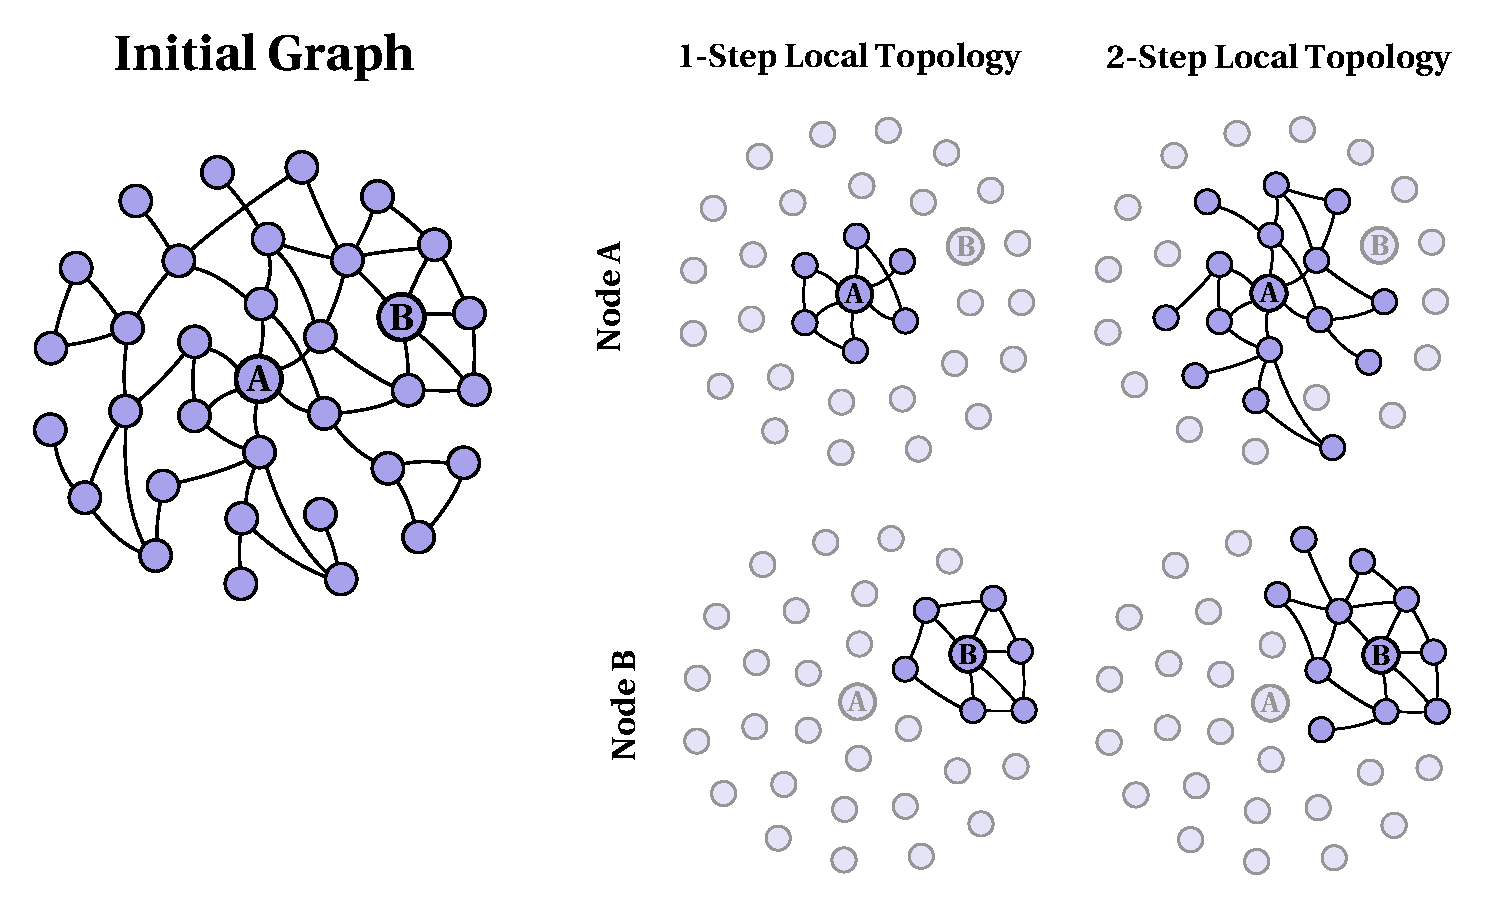
\includegraphics[width=1\textwidth]{../img/fnedRelated/localTopologyFigure.pdf}
  \caption{Illustration showing the 1-step and 2-step local topologies of two nodes in an undirected graph.}
  \label{fig:localTopology}
\end{figure*}


\subsection{Fixed Node Edit Distance (FNED)}

Our first step towards embedding involves defining a distance between the local topologies of nodes; we describe how the distances between nodes can be used for Euclidean embedding in Section~\ref{sec:algos}. The concept of edit distance has been shown to provide an intuitive way to represent distances between abstract structures \cite{riesen2009approximate,reis2004automatic,gao2010survey}. We aim to define an edit distance between the local topologies around nodes in a graph. We call this the Fixed Node Edit Distance (FNED), and define it to be the minimum number of edge insertions (between nodes) or deletions to transform the local topology around one node into the local topology around another node.

An equivalent definition of the FNED, which we refer to as the mapping-overlap formulation, allows for easier computation. Intuitively, for a given mapping between the nodes of a pair of local topologies, we can find the number of edges that ``do not overlap" (i.e. given the mapping, the number of node-pairs that are adjacent in one of the two local topologies but not adjacent in the other). The mapping that yields the minimum number of non-overlapping edges is equivalent to the FNED defined previously (proof omitted).

For a graph $G = \{V,E\}$, let $\Omega_{V}$ be the set of bijections from $V$ to itself (i.e. the set of permutations of $V$). Additionally, let $\Omega_{V, a\rightarrow b}$ be $\Omega_{V}$ restricted to bijections where node $a\in V$ is mapped to node $b\in V$. For all vertices $a,b \in V$, we define the FNED between $a$ and $b$ (given $k$-step local topologies denoted $T_{k}(a)$ and $T_{k}(b)$, respectively), to be
% \begin{equation}
% \begin{split}
% \text{FNED}_{k}(a,b) &= \\ \text{min} & \big|_{m \in \Omega_{V, a\rightarrow b}} d(T_{k}(a), T_{k}(b), m)
% \end{split}
% \end{equation}
\begin{equation}
\text{FNED}_{k}(a,b) = \text{min} \big|_{m \in \Omega_{V, a\rightarrow b}} d(T_{k}(a), T_{k}(b), m)
\end{equation}
where
\begin{equation}
\begin{split}
d(T_{k}(a), & T_{k}(b), m) = \\ 
& \sum_{i=1}^{n} \sum_{j=i}^{n} \Big[ A_{T_{k}(a)}(m(i),m(j)) \oplus A_{T_{k}(b)}(i,j)  \Big]
% & \sum_{i=1}^{n} \sum_{j=i}^{n} A_{T_{k}(a)}(m(i),m(j)) \oplus A_{T_{k}(b)}(i,j)
\end{split}
\end{equation}
where $A_{G}$ denotes the adjacency matrix of graph G. Given adjacency matrices $A_{G_{1}}$ and $A_{G_{2}}$, both of size $n \times n$, we define the XOR operator $\oplus$ to be
\begin{equation}
A_{G_{1}}(i_{1},j_{1}) \oplus A_{G_{2}}(i_{2},j_{2}) = 
\begin{cases}
1 \text{ if } A_{G_{1}}(i_{1},j_{1}) = A_{G_{2}}(i_{2},j_{2}) \\ 
0 \text{ otherwise}
\end{cases}
\end{equation}
We illustrate the two definitions of the FNED and show an example of the distance between two nodes in Figure~\ref{fig:fnedFigure}.

This project is currently concerned only with undirected graphs, with future plans to extend it to directed and other labelled graphs. 


\begin{figure*}[!]
  \centering               
  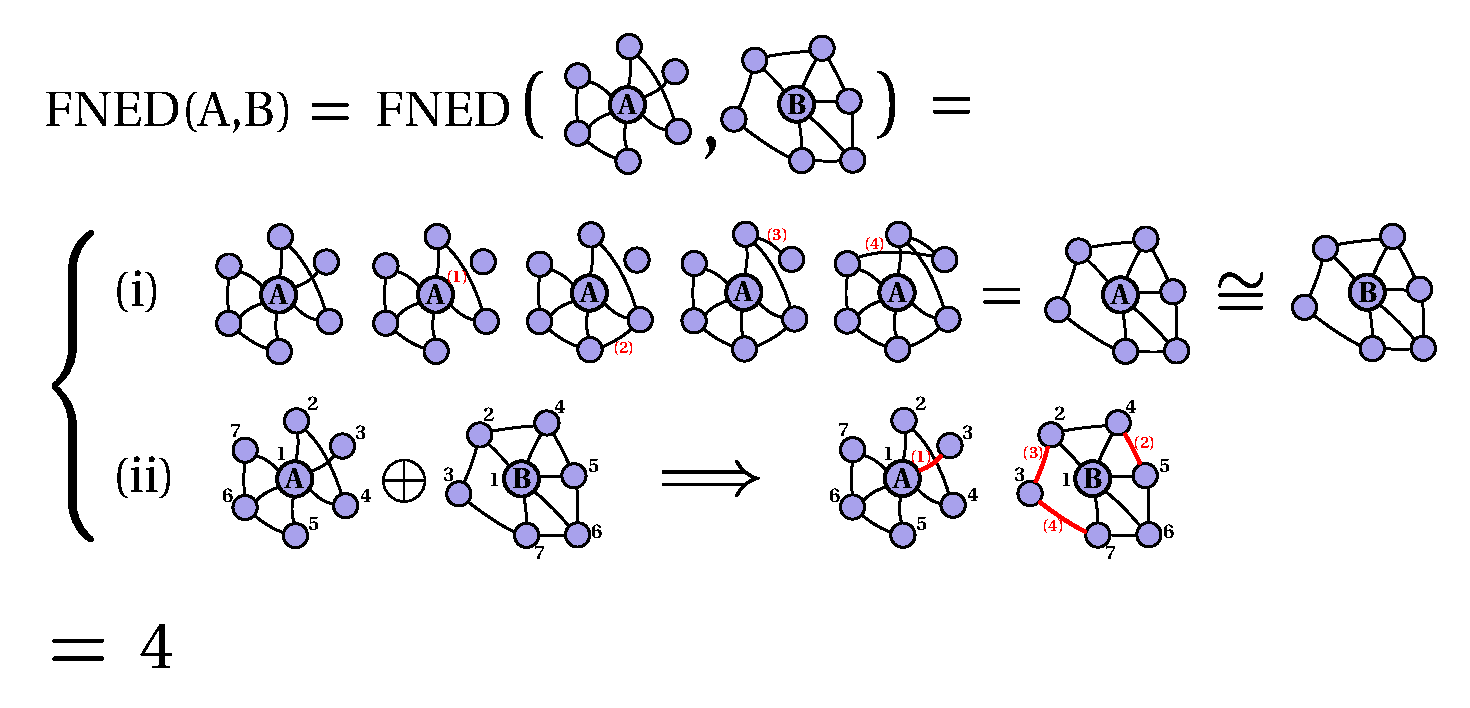
\includegraphics[width=1\textwidth]{../img/fnedRelated/fnedFigure.pdf}
  \caption{Illustration of the FNED between two local topologies. (i) shows the FNED viewed as a sequence of edge edits, while (ii) shows an equivalent definition of the FNED (the mapping-overlap formulation) as a collection of edges that ``do not overlap'' for a given mapping.}
  \label{fig:fnedFigure}
\end{figure*}




\section{Algorithms for Embedding}
\label{sec:algos}
The algorithms in this section describe the process of embedding the nodes of a graph in Euclidean space based on their local topologies.



\subsection{Overview for Embedding Nodes}

Algorithm~\ref{alg:overviewEmbedding} gives an overview of the process of embedding in Euclidean space each node in a graph, based on its local topology.

\begin{algorithm}[!]
\caption{Node Embedding via Local Topologies}
\label{alg:overviewEmbedding}
\begin{algorithmic}[1]
\STATE \textbf{Input:} \\(i) An undirected graph, $G = \{V,E\}$.\\(ii) A local topology step size, $k$.\\(iii) A set of basis nodes, $B \subset V$.
\FOR{each $v \in V$}
\FOR{each $b \in B$}
\STATE Set $\text{Embedding}(v,b) = \text{FNED}_{k}(v,b)$
\ENDFOR
\ENDFOR
\STATE \textbf{Output:} Embedding, the feature matrix where each row is a node, and the set of columns represents the embedding $\in \mathbb{R}^{B}$.
\end{algorithmic}
\end{algorithm}

The embedding into Euclidean space is wholly dependent upon computation of the FNED between the local topologies of the nodes. The following algorithms provide different methods for computing the FNED.


\subsection{Deterministic FNED for Trees}

In Algorithm~\ref{alg:trueFnedTrees} we give a polynomial time algorithm for computing the FNED between nodes in a tree for 2-step local topologies.
\begin{algorithm}[!]
\caption{Deterministic FNED for Trees}
\label{alg:trueFnedTrees}
\begin{algorithmic}[1]
\STATE \textbf{Input:} \\(i) An undirected graph, $G = \{V,E\}$ without loops.\\(ii) Two nodes: $A, B \in V$.
\STATE{Compute $T_{2}(A)$ and $T_{2}(B)$, the local topologies of $A$ and $B$.}
\STATE{$N = \text{max}(|T_{2}(A)|, |T_{2}(B)|)$}
\STATE{Add $N-\text{min}(|T_{2}(A)|, |T_{2}(B)|)$ disconnected ``virtual nodes'' to the local topology with less nodes.}
\FOR{each $a \in T_{2}(A)$ adjacent to $A$}
\FOR{each $b \in T_{2}(B)$ adjacent to $B$}
\STATE Find $n_{a} = \# \{ a' | a' \text{ adjacent to } a \text{ and } a' \neq A \}$
\STATE Find $n_{b} = \# \{ b' | b' \text{ adjacent to } b \text{ and } b' \neq B \}$
\STATE Set $\text{CostMatrix}(a,b) = | n_{a} - n_{b} |$
\ENDFOR
\ENDFOR
\STATE $\text{OptMap}=\text{HungarianAlgorithm}(\text{CostMatrix})$
\STATE $\text{FNED}_{k}(A,B) = \sum_{i=1}^{|T_{2}(A)|} \text{XOR}(i,\text{OptMap}(i))$
\STATE \textbf{Output:} $\text{FNED}_{k}(A,B)$, the fixed node edit distance between $A$ and $B$ for $k$-step local topologies.
\STATE Note 1: HungarianAlgorithm() returns an optimal mapping between nodes adjacent to $A$ and nodes adjacent to $B$ given CostMatrix.
\STATE Note 2: XOR(i,j) returns $|n_{i} - n_{j}|$ (defined on lines 7 and 8) for $i \in T_{2}(A)$ and $j \in T_{2}(B)$.
\end{algorithmic}
\end{algorithm}
% \begin{algorithm}[!]
% \caption{Deterministic True FNED for Trees}
% \label{alg:trueFnedTrees}   % haven't gotten this label to work for some reason
% \begin{algorithmic}[1]
% \STATE \textbf{Input:} \\(i) An undirected graph, $G = \{V,E\}$ without loops.\\(ii) A local topology step size, $k$.\\(iii) Two nodes: $A, B \in V$.
% \STATE{steps $= 0$}
% \FOR{each $a \in V$ adjacent to $A$}
% \FOR{each $b \in V$ adjacent to $B$}
% \IF{steps $= k$}
% \STATE Set $\text{CostMatrix}(a,b) = \text{difference}$
% \ELSE
% \STATE Set $k = k+1$ 
% \STATE Compute CostMatrix for all adjacent nodes.
% \STATE Compute OptimalMap with HungarianAlgorithm.
% \STATE Compute XOR edge distance for given map.
% \ENDIF
% \ENDFOR
% \ENDFOR
% \STATE $\text{OptimalMap}=\text{HungarianAlgorithm}(\text{CostMatrix})$
% \STATE Compute XOR edge distance for given map.
% \STATE \textbf{Output:} $\text{FNED}_{k}(A,B)$, the fixed node edit distance between A and B for $k$-step local topologies.
% \end{algorithmic}
% \end{algorithm}


\subsection{Approximate FNED for Arbitrary Graphs}

Finding an optimal graph matching is not possible in polynomial time for arbitrary graphs. In this section we provide a Markov Chain Monte Carlo (MCMC) -based algorithm to search the combinatorial space of mappings between the nodes of two local topologies. The algorithm follows a directed random walk through the space of permutations of nodes in a local topology.

% \subsubsection{Tree Based Heuristic}

\subsubsection{MCMC for FNED Computation}
Here, we formulate computation of the FNED between nodes as a stochastic combinatorial optimization problem. In Algorithm~~\ref{alg:fnedMcmc} we describe an MCMC algorithm similar to Metropolis-Hastings for sampling the FNED between two nodes in an arbitrary graph.

\begin{algorithm}[!]
\caption{MCMC for FNED in Arbitrary Graphs}
\label{alg:fnedMcmc}
\begin{algorithmic}[1]
\STATE \textbf{Input:} \\(i) An undirected graph, $G = \{V,E\}$.\\(ii) A local topology step size, $k$.\\(iii) Two nodes: $A, B \in V$\\(iv) Maximum sampling iteration, NumIter.
\STATE{Compute $T_{k}(A)$ and $T_{k}(B)$, the $k$-step local topologies of $A$ and $B$.}
\STATE{$N = \text{max}(|T_{k}(A)|, |T_{k}(B)|)$}
\STATE{Add $N-\text{min}(|T_{k}(A)|, |T_{k}(B)|)$ disconnected (degree 0) nodes to the local topology with fewer nodes.}
\STATE{Initialize a mapping $m$ between nodes in $T_{k}(A)$ and nodes in $T_{k}(B)$}
\FOR{$i=1:\text{NumIter}$}
\STATE{$m' = m$}
\STATE{Randomly choose 3 nodes $\in T_{k}(a)$, and randomly permute their mapping in $m'$}
\IF{$d(T_{k}(a), T_{k}(b), m') < d(T_{k}(a), T_{k}(b), m)$}
\STATE{Set $m = m'$}
\STATE{Record $d(T_{k}(a), T_{k}(b), m)$}
\ELSE
\IF{rand() $ < \frac{d(T_{k}(a), T_{k}(b), m)}{d(T_{k}(a), T_{k}(b), m')}$}
\STATE{Set $m = m'$}
\STATE{Record $d(T_{k}(a), T_{k}(b), m)$}
\ENDIF
\ENDIF
\ENDFOR
\STATE $\text{FNED}_{k}(A,B)$ = the minimum $d(T_{k}(a), T_{k}(b), m)$ over $m$ through all iterations.
\STATE \textbf{Output:} $\text{FNED}_{k}(A,B)$, the fixed node edit distance between $A$ and $B$ for $k$-step local topologies.
\STATE{Note 1: $d(T_{k}(a), T_{k}(b), m)$ is defined in Section~\ref{sec:defs}}.
\STATE{Note 2: rand() returns a uniformly distributed random number $\in (0,1)$}
\end{algorithmic}
\end{algorithm}


\section{Experiments}
\label{sec:exp}

% \subsection{Exploring the Embeddings of Nodes in Random Trees}
% This experiment illustrates the embeddings of nodes in synthetically generated random tree graphs. 

\subsection{Graph Clustering with Local Topologies in a Dolphin Social Network}

The dataset in this experiment consists of a social network between a collection of 62 dolphins \cite{bottleNoseDolphinPeople}. An edge was assigned between two dolphins if researchers spotted them traveling in the same group.
\begin{figure*}[!]
  \centering               
  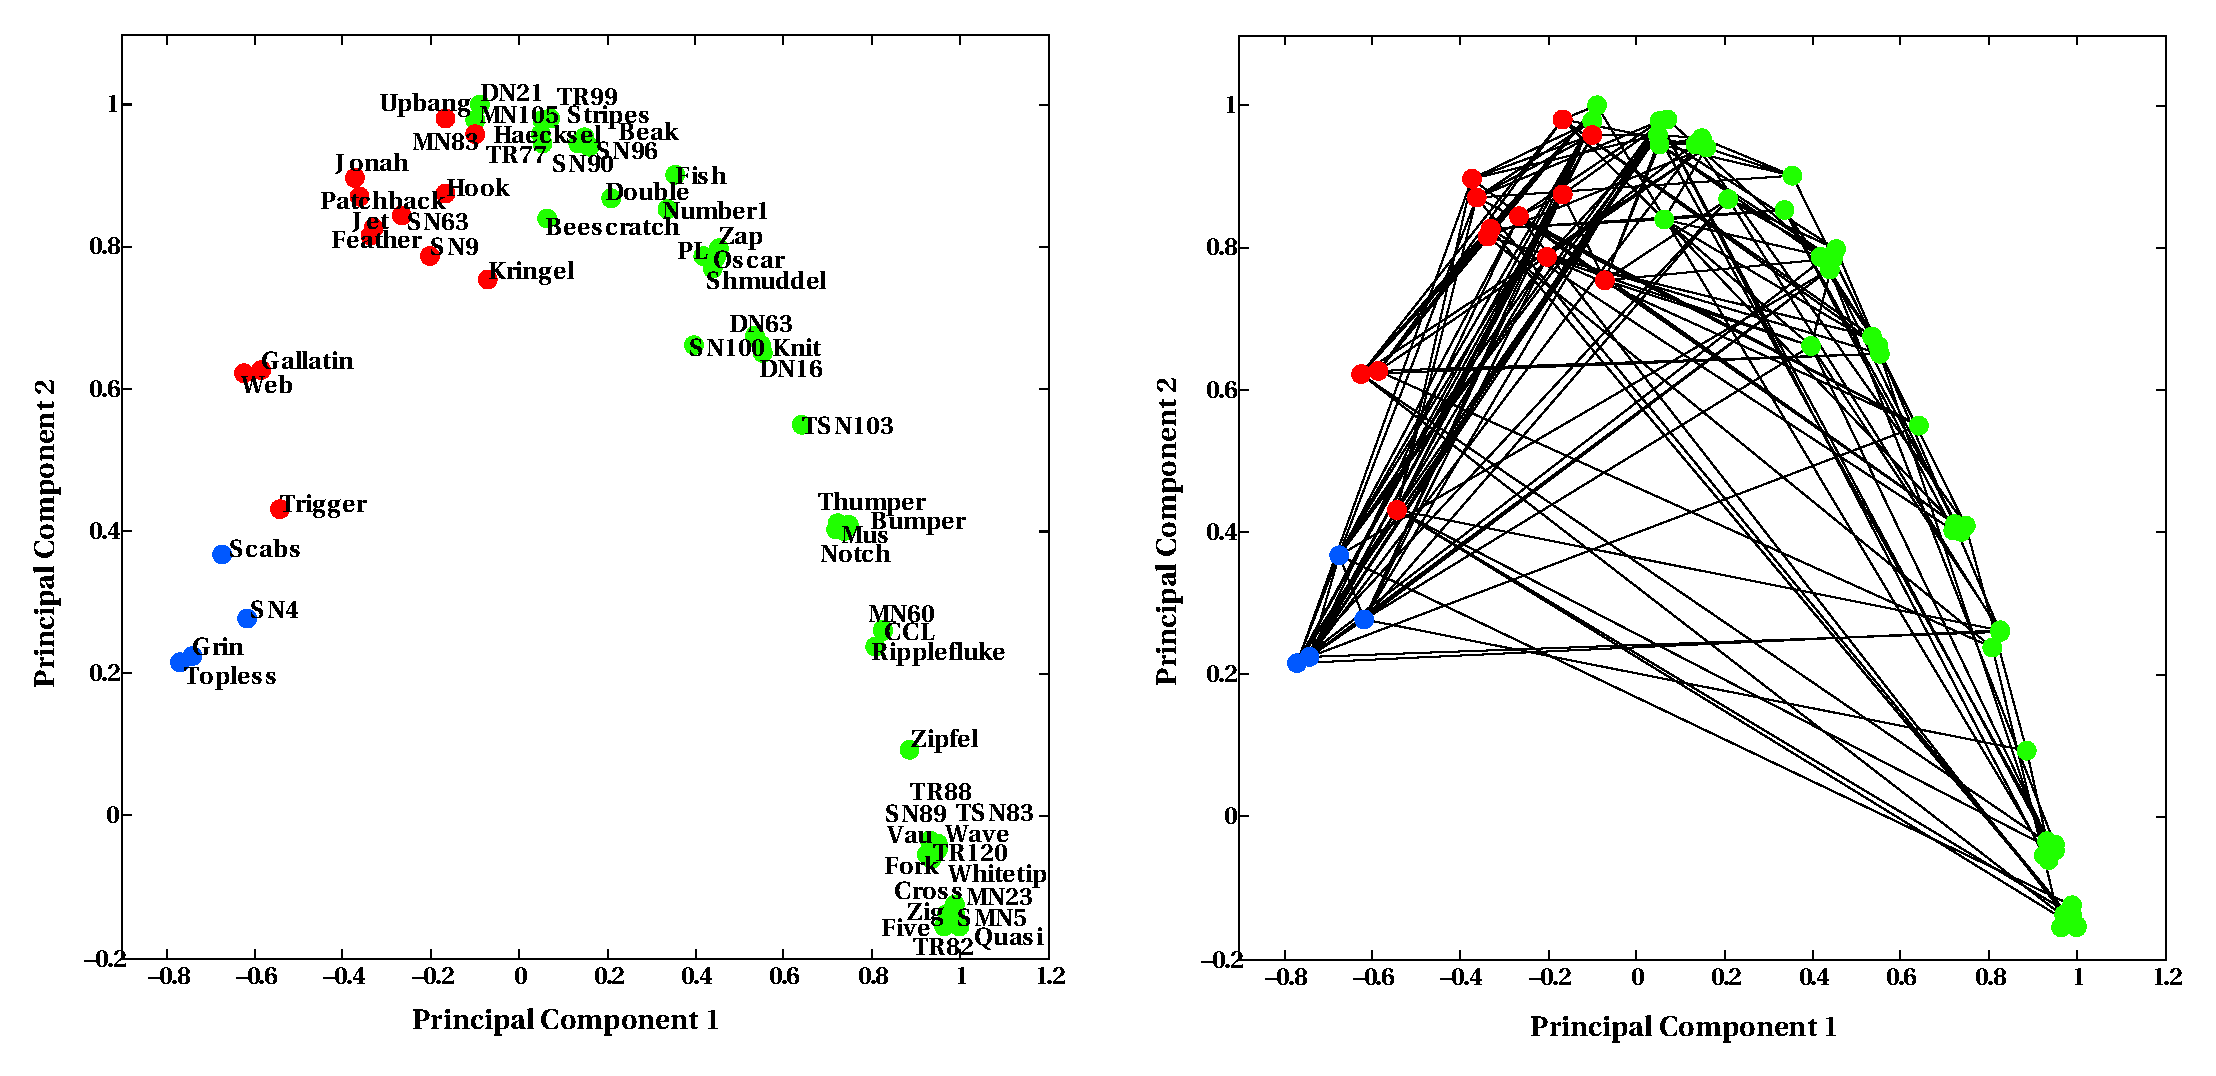
\includegraphics[width=1\textwidth]{../img/demo5_dolphinSocialNetwork/dolphinFigure.pdf}
  \caption{A dolphin social network is shown. The axes denote the first two principal components of the Euclidean embedding of the nodes (i.e. dolphins). Clustering the dolphins (using the $k$-means algorithm) yields three main types of local topologies in this social network, which we can view as clusters of dolphin social behavior. The dolphin's names are shown, as are the edges in the network, and the marker color in both plots denotes each dolphin's cluster assignment.}
  \label{fig:dolphinSocialNetwork}
\end{figure*}

Embedding was performed using the MCMC algorithm to compute the FNED between 1-step local topologies. Aften embedding, the $k$-means algorithm was carried out to perform clustering of the dolphins based on their local topologies. The $k$-means algorithm was initialized at 10 clusters, but returned three clusters as a result. The embedding seems to separate dolphins by their social patterns, and the three clusters might be interpreted as high sociability, medium sociability, and low sociability. Note that the method of node embedding presented in this paper could be viewed as a richer version of node degree, as it yields a high dimensional description of topological structure around a node, while degree yields a very local, 1-dimensional description. Figure~\ref{fig:dolphinSocialNetwork} plots the first two principal components of the node embedding, with marker color denoting the $k$-means cluster assignment (note that $k$-means was performed on the embedded feature vector, not on the principal components). The second plot on this figure shows the dolphin social network graph. Visually, one can see the number of edges decreasing when moving from left to right along the curve.


\subsection{Words in Dickens' David Copperfield with Adjective-Noun Labels}

The dataset in this experiment consists of the 60 most common nouns and adjectives in Charles Dickens' David Copperfield \cite{newman2006finding}. Edges are assigned between words if they appear adjacent to each other at any point in the text.

In this experiment, we hope to show that the embedding method described in this paper yields features that could be used to benefit a supervised machine learning problem; if so, Euclidean local topology features could be added to the features of datasets that are equipped with information about relationships between data elements. In particular, we hope to see some sort of differentiation between the embedding of adjectives and the embedding of the nouns in this dataset.

\begin{figure*}[!]
  \centering               
  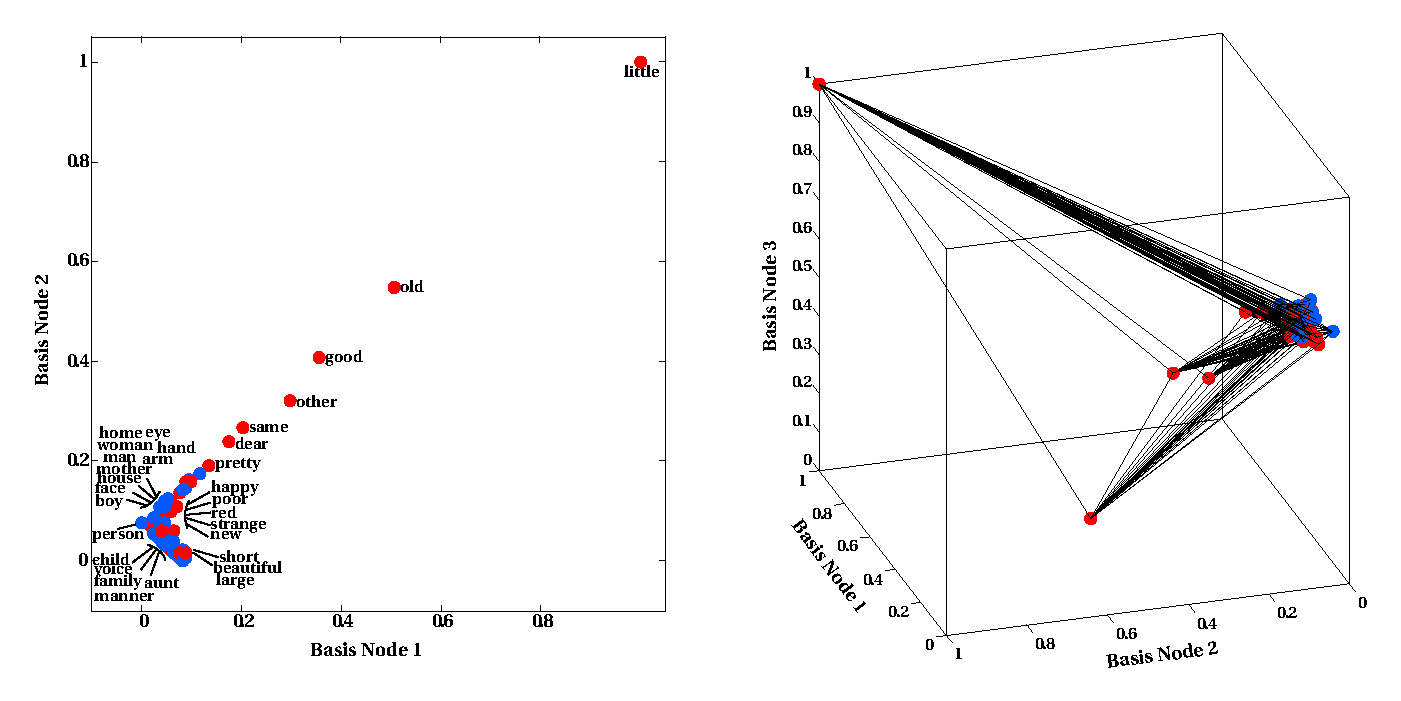
\includegraphics[width=1\textwidth]{../img/demo6_dickensCopperfield/dickensFigure.pdf}
  \caption{The 60 most common adjectives and nouns in Dickens' David Copperfield. Red markers denote adjectives and blue markers denote nouns. Words of different types tend to be embedded in different positions in space.}
  \label{fig:dickensCopperfield}
\end{figure*}

Embedding was performed using the MCMC algorithm to compute the FNED between 1-step local topologies. Figure~\ref{fig:dickensCopperfield} plots the first two dimensions (and first three dimensions on the right) of the embedding feature vectors. A few of the words, along with the graph edges, are shown in the two plots. Adjectives are colored red and nouns are colored blue. From this embedding, we can see that the adjectives and nouns are slightly differentiated in the embedding space. Additionally, a group of adjectives are isolated from the rest of the words.


\subsection{College Football Team Matches with League Labels}

The datset in this experiment consists of the ``matchups'' between 115 college football teams \cite{newman2006finding} in a given season. Edges are assigned between two teams if they play each other during the season. Additionally, this dataset provides a label for each team to the league in which it resides (out of 12 leagues). 

Similar to the previous experiment, we hope to show that the embedding method described in this paper yields features that could be used to benefit a supervised machine learning problem; in particular, we hope to see an embedding that places teams with similar matchup topologies near each other in space. We would guess that teams residing in the same league have similar matchup topologies.

\begin{figure*}[!]
  \centering               
  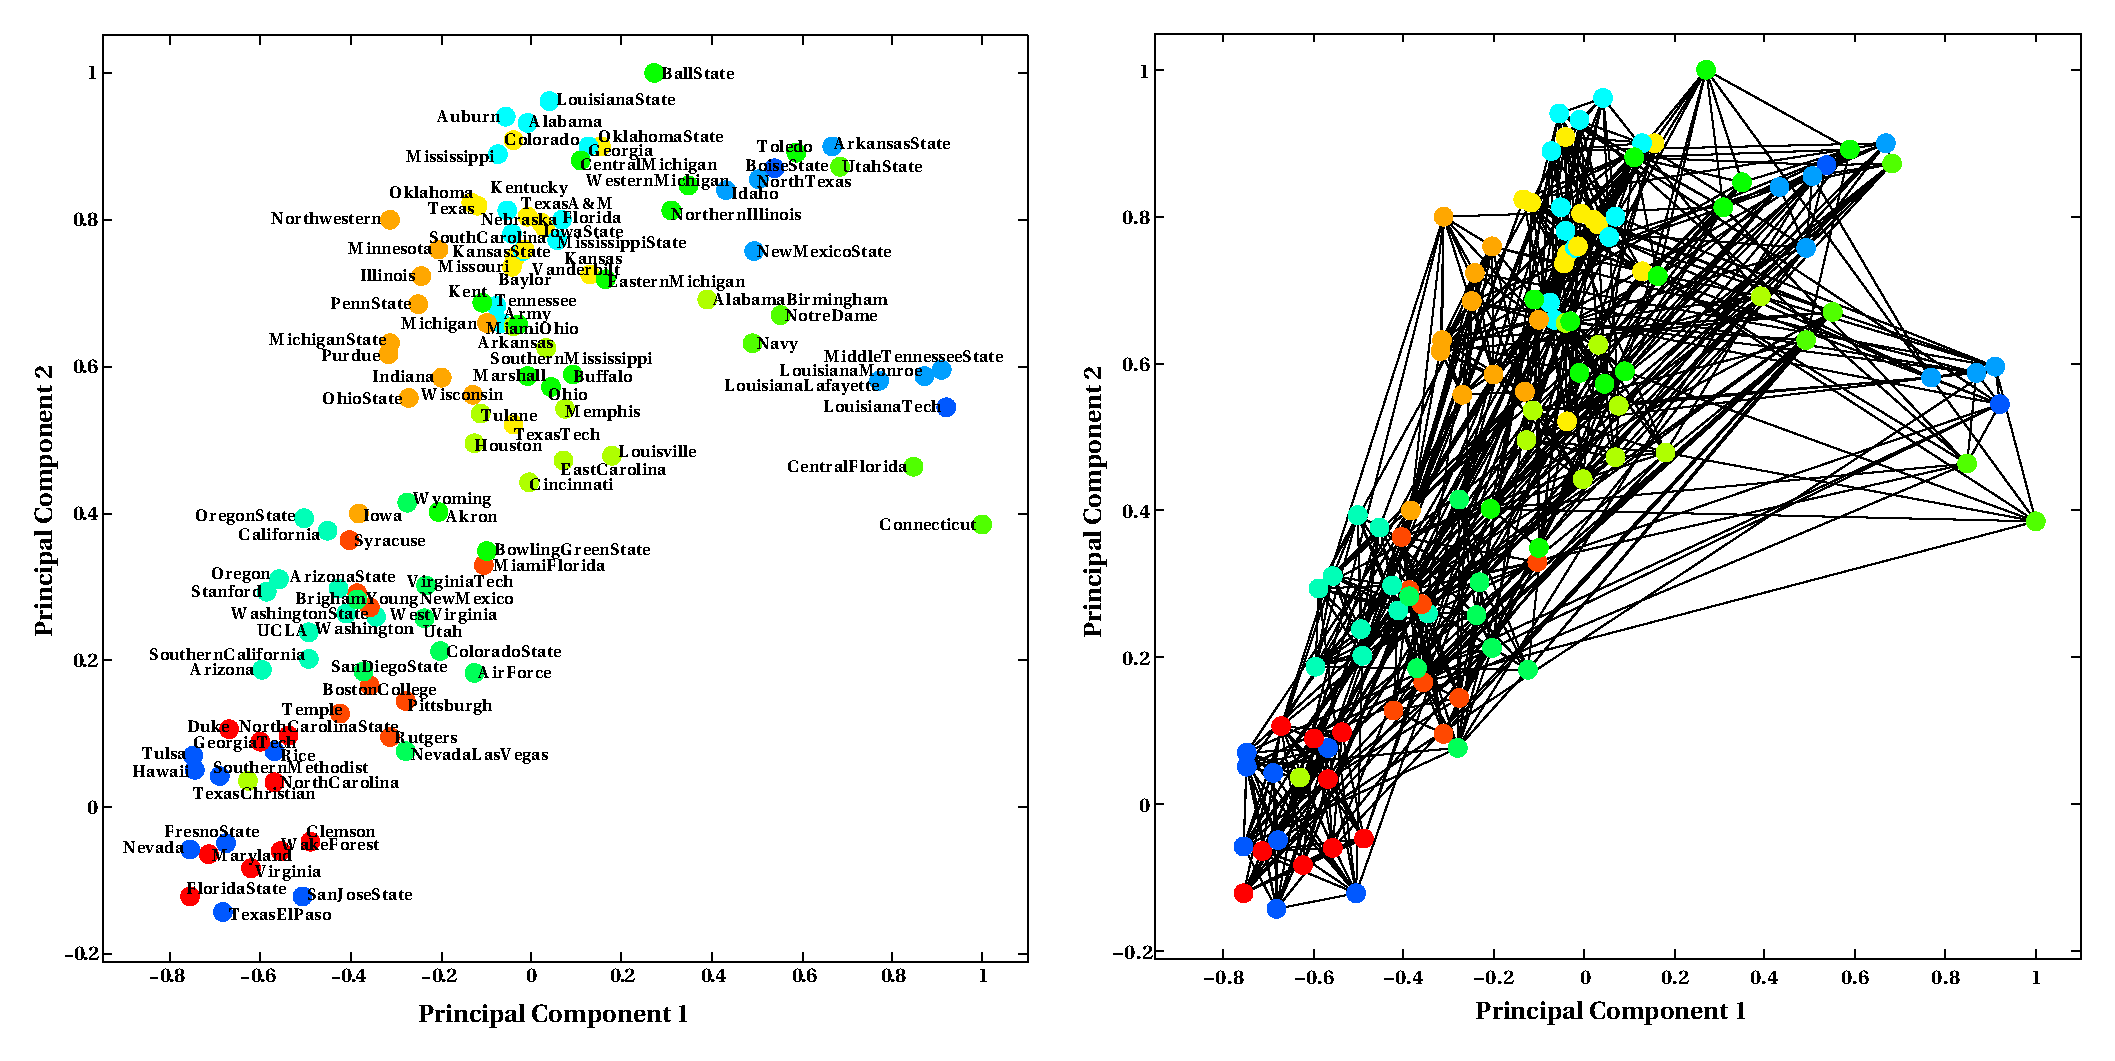
\includegraphics[width=1\textwidth]{../img/demo7_footballTeams/footballFigure.pdf}
  \caption{A network of college football team matchups during a given season is shown. Markers are colored based on the league (out of 12) in which the associated team resides. Teams belonging to the same league tend to be embedded similarly, as do teams from similar geographic locations.}
  \label{fig:footballTeams}
\end{figure*}

Embedding was performed using the MCMC algorithm to compute the FNED between 1-step local topologies. Figure~\ref{fig:footballTeams} shows the first two principal components of the Euclidean embedding. This figure also shows school name for each team and the matchup graph edges. In both plots, color denotes league assignment. We find that the embedding often places football teams from the same league at similar points in space. We also find a number of other points of interest, such as places where schools from similar geographic locations are embedded similarly (even for similar geographic schools in different leagues).


\section{Conclusion}
\label{sec:conclusion}

We have introduced a method for representing the local topology around a node in Euclidean space by defining the $k$-step local topology and fixed node edit distance between nodes. Additionally, we have provided two algorithms for computing the FNED between nodes of different types of graphs, and have demonstrated this embedding on three publically available datsets. Our demonstrations have shown that the Euclidean local topology features can be used alone to perform graph clustering of nodes into groups with similar local topologies, or can provide additional features for datasets equipped with relationships between their elements, in order to benefit a supervised learning task. 


\begin{small}
\bibliographystyle{plainnat}
\bibliography{paper_refs} 
\end{small}

\end{document}


% \begin{figure}[h]
%   \centering             
%   \subfloat[]{\includegraphics[width=0.32\textwidth]{../img/kmeans_2.pdf}}
%   \hspace{1mm}
%   \subfloat[]{\includegraphics[width=0.32\textwidth]{../img/kmeans_3.pdf}}
%   \hspace{1mm}
%   \subfloat[]{\includegraphics[width=0.32\textwidth]{../img/kmeans_4.pdf}}
%   \caption{K-means clustering results on the 5 frame sequences of cell speeds extracted from time lapse microscopy video data. The mean speed (over all sequences) is subtracted from each value of each sequence for detrending. Speed in relative units is displayed on the y axis. The color of each sequence denotes its cluster assignment. Results are shown for $K=2$ (a), $K=3$ (b), and $K=4$ (c).}
%   \label{fig:kmeans}
% \end{figure}


% \begin{figure}[h]
%   \centering             
%   \subfloat[]{\includegraphics[width=0.28\textwidth]{../img/control.pdf}}
%   \hspace{1mm}
%   \subfloat[]{\includegraphics[width=0.28\textwidth]{../img/raromix.pdf}}
%   \hspace{1mm}
%   \subfloat[]{\includegraphics[width=0.28\textwidth]{../img/well6.pdf}}
%   \caption{Three example frames from the benchmark cell video datasets used in experiments one (a), two (b), and three (c). }
%   \label{fig:cell_imgs}
% \end{figure}
